\documentclass[tikz,border=12pt]{standalone}
\usepackage{amsmath,amssymb}
\usetikzlibrary{calc}

\begin{document}
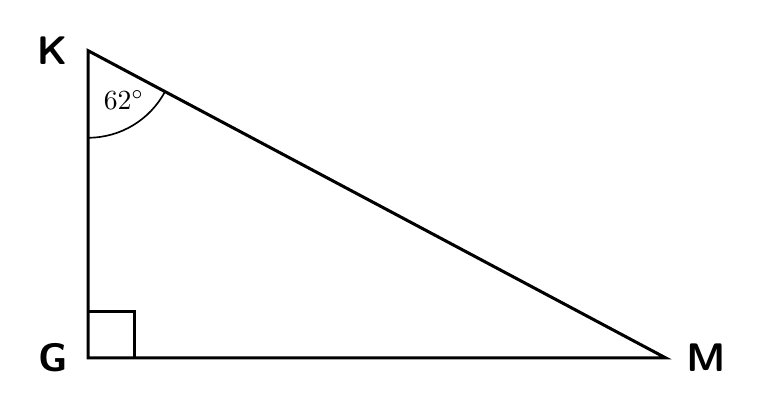
\begin{tikzpicture}[scale=1.3]
    % Triangle dimensions: KG = 3.0, GM = 3.0 * tan(62 deg) = 3.0 * 1.8807 = 5.642
    \pgfmathsetmacro{\kg}{3.0}
    \pgfmathsetmacro{\gm}{5.64}
    
    \coordinate (G) at (0, 0);
    \coordinate (K) at (0, \kg);
    \coordinate (M) at (\gm, 0);
    
    % Draw triangle
    \draw[line width=1.1pt] (G) -- (M) -- (K) -- cycle;
    
    % Vertices labels in bold sans-serif
    \node[left=4pt, font=\Large\sffamily\bfseries] at (G) {G};
    \node[left=4pt, font=\Large\sffamily\bfseries] at (K) {K};
    \node[right=4pt, font=\Large\sffamily\bfseries] at (M) {M};
    
    % Right angle symbol at G
    \draw[line width=1.0pt] (0, 0.45) -- (0.45, 0.45) -- (0.45, 0);
    
    % Angle arc at K: from vertical downward (-90) towards hypotenuse (-28)
    \draw[semithick] ($(K) + (270:0.85)$) arc (270:332:0.85);
    \node[font=\bfseries] at (0.35, {\kg - 0.48}) {$62^\circ$};
    
\end{tikzpicture}
\end{document}
